% --------------------------
% ---- DECLARE PACKAGES ----
% --------------------------
% Sintesi in 10 pagine della tesi. Stesso impianto del progetto madre
% (book, pdflatex, biblatex + biber, minted): si compila con
%   latexmk -pdf -shell-escape -aux-directory=auxil -output-directory=out main.tex
% eseguito dentro questa cartella. Testo condensato dall'originale,
% senza modificare i file della tesi.
\documentclass[a4paper, oneside, openright]{book}

% PDF/A-2b
\usepackage[a-2b]{pdfx}

\usepackage[T1]{fontenc} % Font encoding, T1 = it
\usepackage{lmodern}
\usepackage{multicol} % Per il frontespizio
\usepackage[utf8]{inputenc} % Input encoding
\usepackage[english,italian]{babel} % Lingua principale italiana, con parti in inglese
\usepackage{minted} % Per i blocchi di codice
\usepackage{csquotes} % Dipendenza di babel e biblatex
\usepackage{graphicx} % Immagini esterne

\usepackage{setspace}
\onehalfspacing % interlinea 1.5

\usepackage[parfill]{parskip} % Disabilita l'indentazione dopo essere andati a capo
\usepackage{titlesec}
\usepackage{float}
\usepackage{booktabs}
\usepackage{longtable}
\usepackage{tabularx}
\usepackage{multirow}
\usepackage{enumitem}
\usepackage{amsmath}
\usepackage{amssymb}

% Colonne di tabella a bandiera
\newcolumntype{L}{>{\raggedright\arraybackslash}X}
\newcolumntype{P}[1]{>{\raggedright\arraybackslash}p{#1}}
\newcolumntype{B}[1]{>{\raggedright\arraybackslash\bfseries}p{#1}}

% Percorso immagini: "../" serve al Frontespizio, che punta a Immagini/...
\graphicspath{{../}{../Immagini/}{../Immagini/Sessioni/}{../Immagini/Screenshot/}}

% Diagrammi TikZ
\usepackage{tikz}
\usepackage{pgfplots}
\pgfplotsset{compat=1.18}
\usetikzlibrary{shapes.geometric, shapes.multipart, arrows, arrows.meta,
                positioning, fit, backgrounds, calc, chains, automata,
                decorations.pathreplacing}
\tikzstyle{startstop} = [rectangle, rounded corners, minimum width=3cm, minimum height=1cm,text centered, draw=black, fill=red!30]
\tikzstyle{io} = [trapezium, trapezium left angle=70, trapezium right angle=110, minimum width=3cm, minimum height=1cm, text centered, draw=black, fill=blue!30]
\tikzstyle{process} = [rectangle, minimum width=3cm, minimum height=1cm, text centered, draw=black, fill=orange!30]
\tikzstyle{decision} = [diamond, minimum width=3cm, minimum height=1cm, text centered, draw=black, fill=green!30]
\tikzstyle{arrow} = [thick,->,>=stealth]

% Stili per i diagrammi
\tikzset{
  layer/.style   = {rectangle, rounded corners=3pt, draw=black!70, thick,
                    align=center, inner sep=6pt, minimum height=1cm},
  comp/.style    = {rectangle, rounded corners=2pt, draw=black!60,
                    fill=white, align=center, font=\footnotesize,
                    inner sep=4pt, minimum height=0.8cm},
  extern/.style  = {rectangle, dashed, draw=black!60, align=center,
                    font=\footnotesize, inner sep=4pt},
  ucase/.style   = {ellipse, draw=black!70, align=center,
                    font=\footnotesize, inner sep=2pt, minimum width=2.6cm},
  flow/.style    = {-{Latex[length=2mm]}, thick},
  flowdash/.style= {-{Latex[length=2mm]}, thick, dashed},
  tile/.style    = {rectangle, draw=black!55, fill=black!2, thin},
  cellgrid/.style= {draw=black!35, thin, dash pattern=on 1.2pt off 1.2pt},
  pin/.style     = {circle, fill=black!75, draw=none, inner sep=0pt,
                    minimum size=3pt},
  bubble/.style  = {circle, draw=black!65, fill=black!12, thick,
                    inner sep=0pt, font=\scriptsize},
  tick/.style    = {black!70, thin},
  band/.style    = {rectangle, draw=black!55, fill=black!6, rounded corners=1pt}
}

% Captions
\usepackage[font=scriptsize, skip=5pt, justification=centering]{caption}

\usepackage[backend=biber, style=numeric, backref=true, defernumbers=true]{biblatex}

% Per sitografia
\setcounter{biburlnumpenalty}{7000}
\setcounter{biburlucpenalty}{7000}
\setcounter{biburllcpenalty}{7000}
\renewcommand*{\bibfont}{\small} % Sitografia compatta per le 10 pagine

\usepackage[immediate]{silence}
\WarningFilter[temp]{latex}{Command}
\usepackage{sectsty}
\DeactivateWarningFilters[temp]

% Impaginazione e margini
\usepackage[fontsize=12pt]{scrextend} % dimensione font

% footmisc
\usepackage[bottom]{footmisc}
\usepackage{hyperref}
\usepackage{subcaption}

% Sperimentali
\WarningFilter{microtype}{Unable to apply patch `footnote'}
\usepackage{microtype}

\usepackage[top=3.5cm,bottom=3.5cm,left=3.5cm,right=3.5cm]{geometry}

% Aspetto liste
\setminted{
  fontsize=\small,
  breaklines=true,
  breakanywhere=true,
  tabsize=2,
  frame=lines,
  framesep=6pt,
  xleftmargin=0pt
}
\renewcommand{\listingscaption}{Listato}
\renewcommand{\listoflistingscaption}{Elenco dei listati}

% ------------------------
% ---- DOCUMENT SETUP ----
% ------------------------
\pagestyle{plain}
\raggedbottom

\titleformat{\chapter}[display]
{\normalfont\huge\bfseries}{\chaptertitlename\ \thechapter}{10pt}{\LARGE}
\titlespacing*{\chapter}{0pt}{0pt}{20pt}
\chaptertitlefont{\fontsize{22pt}{30pt}\selectfont}

% Titoli
\sectionfont{\raggedright}
\subsectionfont{\raggedright}
\subsubsectionfont{\raggedright}

\hypersetup{
    colorlinks,
    citecolor=black,
    filecolor=black,
    linkcolor=black,
    urlcolor=black
}

\renewcommand{\footnotesize}{\fontsize{11pt}{13pt}\selectfont} % Imposta la dimensione del testo delle footnotes
\setlength{\footnotesep}{0.5cm} % Imposta lo spazio fra le singole footnotes
\setlength{\skip\footins}{1.5cm} % Imposta lo spazio fra il corpo e le footnotes

\DeclareUnicodeCharacter{02BC}{}

% ------------------------
% ---- DOCUMENT START ----
% ------------------------
\addbibresource{../bibliography.bib} % Bibliografia
\begin{document} % Inizio documento
\hypersetup{pageanchor=false}
\frontmatter
\begin{titlepage}
\begin{figure}[!htb]
    \centering
    
\includegraphics[width=5cm]{Immagini/uninsubria-logo}
\end{figure}

\begin{center}
    \Large{\textbf{UNIVERSITÀ DEGLI STUDI DELL'INSUBRIA}}
    \vspace{3mm}
    \\ \normalsize{DIPARTIMENTO DI SCIENZE TEORICHE E APPLICATE}
    \vspace{6mm}
    \\ \normalsize{CORSO  DI STUDIO TRIENNALE  IN}
    \\  \normalsize{\textbf{INFORMATICA}}
    \vspace{13mm}
    % \\ \normalsize{Tesi  di Laurea}
\end{center}

\vspace{10mm}
\begin{center}
    \LARGE{\textbf{Progettazione e sviluppo di un'applicazione mobile cross-platform in Flutter per la geolocalizzazione e la gestione personalizzata di centri dermatologici}}
\end{center}

\vspace*{\fill}

\begin{minipage}[t]{1\textwidth}
    \begin{multicols}{2}
    	{\normalsize{\textbf{Relatore:}}{\normalsize\vspace{1mm}
        \\ \normalsize{Prof. Ignazio Gallo }}} \\

        {\normalsize{\textbf{Correlatori:}}{\normalsize\vspace{1mm}
        \\ \normalsize{Andrea Carugno, Mattia Gatti}}} \\
        
         %\columnbreak
         %\columnbreak

         \begin{flushright}
            {\normalsize{\textbf{Tesi di Laurea di:}}{\normalsize\vspace{1mm}
            \\ \normalsize{Gabriele Caretti}\\
            \normalsize{Matricola  756564 }}} \\
         \end{flushright}
    \end{multicols}
\end{minipage}

\begin{center}
    {\normalsize{\textbf{Anno accademico:}}{\normalsize\vspace{1mm}
    \\ \normalsize{2025/2026}}}  
\end{center}

\end{titlepage}
 % PAGINA FRONTESPIZIO, identica alla tesi
\tableofcontents  % Genera l'indice
\mainmatter
\hypersetup{pageanchor=true}
\setcounter{chapter}{1} % Sezioni numerate 1.1--1.8 senza testata "Capitolo 1"

% ------------------
% ---- SINTESI -----
% ------------------
\chapter*{Tesi in sintesi}\label{ch:sintesi}
\addcontentsline{toc}{chapter}{Tesi in sintesi}

\section{Contesto clinico}\label{sec:sintesi-contesto}

La dermatite atopica e la psoriasi condividono una caratteristica che pesa
pi\`u di quanto si potrebbe pensare: non guariscono.
Sono patologie infiammatorie croniche recidivanti, in cui fasi di remissione
e fasi di riacutizzazione si alternano nel corso di anni o di decenni
\cite{weidingerAD, griffithsPsoriasis}.
Chi ne \`e affetto non ha bisogno di una visita isolata, ma di un percorso:
controlli periodici, aggiustamenti della terapia e, in una parte dei casi,
trattamenti che possono essere prescritti soltanto da strutture autorizzate.

La dermatite atopica \`e legata a un difetto della barriera cutanea con
risposta di tipo 2 ed esordio nell'infanzia; la psoriasi all'asse
interleuchina-23 e linfociti T-helper 17, con placche eritematose e possibili
manifestazioni articolari.
La conseguenza organizzativa \`e che le due patologie non vengono seguite
necessariamente dalle stesse strutture, e un elenco che non distingua i due
casi costringe l'utente a verificare struttura per struttura.

L'Organizzazione Mondiale della Sanit\`a ha riconosciuto il ritardo
diagnostico e le difficolt\`a di accesso come problemi di salute pubblica
\cite{whoPsoriasis}, e il Piano Nazionale della Cronicit\`a indica
continuit\`a assistenziale e presa in carico territoriale come punti di
miglioramento \cite{pianoCronicita}.
La domanda concreta: dove si trova il centro pi\`u vicino che segue la mia
patologia, e come ci arrivo?
Due portali censiscono i centri italiani delle due patologie
\cite{dermatopia, viciniDiPelle} e sono un buon punto di partenza; restano
per\`o pagine web desktop, con ricerca per regione o provincia e senza
nozione di distanza dall'utente.
Uno smartphone invece conosce la propria posizione, mostra una mappa, avvia
la navigazione e conserva dati anche offline: da questa asimmetria nasce il
progetto, un'applicazione che rende interrogabili per posizione dati gi\`a
pubblici.

\section{Obiettivi e limiti}\label{sec:sintesi-obiettivi}

L'obiettivo generale \`e la progettazione e la realizzazione di
un'applicazione mobile cross-platform, sviluppata con il framework Flutter,
che permetta di individuare su mappa i centri dermatologici italiani
dedicati alle due patologie e di integrarli con voci inserite dall'utente.
In termini operativi:
\begin{itemize}[itemsep=2pt]
  \item Acquisire gli elenchi da sorgenti pubbliche, senza un nuovo
  archivio;
  \item Normalizzarli in un'unica rappresentazione interna, gestendo record
  incompleti o malformati;
  \item Mostrarli su mappa interattiva con clustering automatico nelle aree
  urbane, filtri per patologia e raggio, ordinamento per distanza geodetica
  e ricerca per indirizzo via geocodifica;
  \item Integrare preferiti e centri personalizzati sul dispositivo, con le azioni
  successive (navigazione, chiamata, email, condivisione) e cache
  persistente per l'uso offline.
\end{itemize}
Definendo i limiti del progetto: l'applicazione non formula diagnosi n\'e
valutazioni cliniche, non prevede autenticazione n\'e profili utente e non
trasmette all'esterno alcun dato personale; non include un backend dedicato
e si basa su servizi pubblicamente disponibili.

\section{Strumenti esistenti}\label{sec:sintesi-limiti}

Dermatopia offre un elenco di centri tramite servizio web pubblico, mentre
Vicini di Pelle pubblica una mappa delle strutture di riferimento costruita
con un plugin cartografico WordPress.
Entrambe risolvono la parte pi\`u complessa, il censimento, che \`e un
lavoro redazionale continuo: il progetto non tenta di costruire un proprio
archivio e assume queste sorgenti come dato di partenza, concentrandosi su
ci\`o che manca, cio\`e l'accesso mobile e georeferenziato.
Dall'analisi emergono i limiti che hanno guidato i requisiti:
\begin{itemize}[itemsep=2pt]
  \item Navigazione per suddivisione amministrativa e non per prossimit\`a;
  \item Posizione dell'utente inutilizzata: nessuna distanza n\'e raggio;
  \item Schermi piccoli penalizzati e azioni successive solo per copia
  manuale;
  \item Nessuna modalit\`a offline e nessun contributo dell'utente: da qui i
  centri personalizzati, nella stessa mappa di quelli remoti.
\end{itemize}

\section{Mappe, geocodifica e framework}\label{sec:sintesi-mappe}

La scelta del provider condiziona costi, licenze e codice.
Sono state valutate tre alternative: Google Maps Platform, con la migliore qualit\`a
ma chiave soggetta a fatturazione con modello a consumo oltre la soglia
gratuita \cite{googleMapsPricing}; Mapbox, con mappe vettoriali e modello
analogo; OpenStreetMap, i cui dati sono sotto licenza Open Database License
\cite{osmCopyright}, integrato in Flutter da
\texttt{flutter\_map}, che disegna i \textit{tile} \cite{flutterMapPkg}.
Rispetto ai primi due, che richiedono credenziali e hanno bassa
sostituibilit\`a, il terzo non ha costi diretti n\'e credenziali, offre alta
sostituibilit\`a e marker totalmente personalizzabili.

Si è quindi scelto OpenStreetMap con \texttt{flutter\_map}: non solo
per i costi, ma perch\'e i marker sono widget Flutter, e il clustering si
costruisce con gli stessi strumenti del resto dell'interfaccia.
I compromessi: i \textit{tile} pubblici vietano usi massivi e impongono
identificativo e caching \cite{osmTilePolicy}, e la grafica raster non \`e
ai livelli di quella vettoriale offerta dalle alternative commerciali.
La visualizzazione segue lo schema \emph{slippy map}: proiezione Web
Mercator e tasselli indicizzati da zoom, colonna e riga, con raddoppio per
lato a ogni zoom \cite{slippyMap}, relazione ripresa dal dimensionamento
delle celle del clustering.
La ricerca usa Nominatim, con al massimo una richiesta al secondo e invito
al caching \cite{nominatimPolicy}: da qui il \textit{debounce} sulla
digitazione.
Per soddisfare il requisito di utilizzare una singola base di codice sia per iOS che per Android, si è scelto Flutter con Dart
\cite{flutterDocs}.%: motore di disegno proprio, risultato prevedibile e
%controllo sui marker al variare dello zoom.

\section{Requisiti e attori}\label{sec:sintesi-requisiti}

Il destinatario \`e una persona, per esempio chi \`e affetto dalle due
patologie ma anche un familiare o un dottore, che usa lo smartphone spesso
con una sola mano e non inserisce dati clinici.
Da qui: nessuna registrazione e controlli nella met\`a inferiore dello
schermo, a portata di pollice.
Gli attori secondari sono i servizi di elenco, la geocodifica, i tile, il
sistema operativo per posizione e permessi, e le app esterne per
navigazione, chiamata, email e condivisione.

I requisiti funzionali prevedono: download dagli elenchi con
\textit{fallback} sulla sorgente secondaria, normalizzazione, scarto dei
record senza coordinate senza bloccare gli altri e cache locale;
mappa con marker, clustering con conteggio e scomposizione
all'avvicinamento; posizione richiesta solo all'uso, non bloccante;
ricerca con suggerimenti; %dopo pausa di digitazione;
filtri combinabili per patologia e raggio con elenco ordinato per distanza
geodetica; centri personalizzati validati, persistenti e distinguibili, pi\`u
preferiti; scheda dei marker e delega di navigazione, chiamata, email e
condivisione.

\section{Architettura e interfaccia}\label{sec:sintesi-architettura}

Non \`e stato realizzato alcun backend: l'applicazione interroga
direttamente elenchi terzi, normalizzati e conservati sul dispositivo.
Resta autonoma, ma \`e esposta a ogni
variazione di formato delle fonti e deve considerare l'irraggiungibilit\`a di una
sorgente.
L'organizzazione interna segue tre livelli sovrapposti, in figura
\ref{fig:sintesi-architettura}: presentazione (mostra e inoltra i gesti),
logica (visibilit\`a, clustering, permessi, validazione) e accesso ai dati.
%unico a conoscere la forma originaria delle sorgenti.

\begin{figure}[H]
\centering
\begin{tikzpicture}[scale=0.64, transform shape, font=\footnotesize]
\node[layer, minimum width=10.6cm, minimum height=2.1cm, fill=black!3] at (5.3,8.2) {};
\node[anchor=north west, font=\scriptsize\bfseries] at (0.15,9.2) {Presentazione};
\node[comp, text width=2.1cm] at (1.50,7.9) {Mappa e livelli};
\node[comp, text width=2.1cm] at (4.05,7.9) {Controlli mappa};
\node[comp, text width=2.1cm] at (6.60,7.9) {Barra di ricerca};
\node[comp, text width=2.1cm] at (9.15,7.9) {Schede e moduli};
\node[layer, minimum width=10.6cm, minimum height=2.1cm, fill=black!3] at (5.3,5.2) {};
\node[anchor=north west, font=\scriptsize\bfseries] at (0.15,6.2) {Logica applicativa};
\node[comp, text width=2.1cm] at (1.50,4.9) {Selezione e clustering};
\node[comp, text width=2.1cm] at (4.05,4.9) {Filtri e prossimit\`a};
\node[comp, text width=2.1cm] at (6.60,4.9) {Permessi e posizione};
\node[comp, text width=2.1cm] at (9.15,4.9) {Validazione e link};
\node[layer, minimum width=10.6cm, minimum height=2.1cm, fill=black!3] at (5.3,2.2) {};
\node[anchor=north west, font=\scriptsize\bfseries] at (0.15,3.2) {Accesso ai dati};
\node[comp, text width=2.9cm] at (2.0,1.9) {Acquisizione remota};
\node[comp, text width=2.9cm] at (5.3,1.9) {Normalizzazione};
\node[comp, text width=2.9cm] at (8.6,1.9) {Cache e persistenza};
\draw[{Latex[length=2mm]}-{Latex[length=2mm]}, thick] (2.6,7.1) -- (2.6,6.3);
\draw[{Latex[length=2mm]}-{Latex[length=2mm]}, thick] (8.0,7.1) -- (8.0,6.3);
\draw[{Latex[length=2mm]}-{Latex[length=2mm]}, thick] (2.6,4.1) -- (2.6,3.3);
\draw[{Latex[length=2mm]}-{Latex[length=2mm]}, thick] (8.0,4.1) -- (8.0,3.3);
\node[extern, text width=2.9cm, anchor=west] at (11.3,7.9) {Tile OpenStreetMap};
\node[extern, text width=2.9cm, anchor=west] at (11.3,5.9) {Posizione del dispositivo};
\node[extern, text width=2.9cm, anchor=west] at (11.3,3.9) {Navigazione, telefono, posta};
\node[extern, text width=2.9cm, anchor=west] at (11.3,1.9) {Elenchi e geocodifica};
\draw[flowdash] (10.6,7.9) -- (11.3,7.9);
\draw[flowdash] (10.6,5.9) -- (11.3,5.9);
\draw[flowdash] (10.6,3.9) -- (11.3,3.9);
\draw[flowdash] (10.6,1.9) -- (11.3,1.9);
\end{tikzpicture}
\caption{Architettura a tre livelli e sistemi esterni (sintesi).}
\label{fig:sintesi-architettura}
\end{figure}

Gli scambi fra livelli sono bidirezionali, quelli verso l'esterno sono solo in
uscita: l'applicazione interroga o delega, nessuno la contatta.
Per lo stato non si usa alcuna libreria: bastano stato locale ed eventi,
con l'elenco dei visibili separato e osservabile, cos\`i
il suo ridisegna altera solo il livello dei marker; il ricalcolo su
viewport in movimento \`e rinviato alla fine del gesto.
L'interfaccia \`e una schermata intera senza nuove schermate: dettagli,
elenchi e moduli salgono dal basso coprendo solo una parte della mappa.
I comandi stanno sopra la mappa e si nascondono durante la ricerca, che non
ridimensiona la schermata.
I centri pubblici arrivano gi\`a selezionati per patologia; quelli personali
portano la patologia come attributo con filtro a schermo, senza
duplicazioni.

\section{Dati, mappa e clustering}\label{sec:sintesi-dati}

Le sorgenti differiscono in forma, nomi dei campi e struttura: una espone
i contatti in campi dedicati, l'altra in HTML da cui estrarli.
La normalizzazione riconduce i nomi con catene di \textit{alias},
recupera i contatti con \textit{regex} e ripara le coordinate con doppi
separatori; i record senza coordinate valide vengono scartati senza fermare gli
altri.

L'interrogazione prevede una fonte per patologia: la seconda, esposta da
CMS, seleziona la categoria, richiede header specifici e pulizia del
BOM, con \textit{timeout}. %di quarantacinque secondi.
Se la fonte non risponde, scatta il \textit{fallback};
l'altra patologia si precarica in \textit{background}, cos\`i il selettore
a due posizioni diventa istantaneo.
Il salvataggio utilizza un archivio chiave-valore JSON: due chiavi per le
cache e una con suffisso di versione per i centri personalizzati.
All'avvio la mappa utilizza la cache e poi aggiorna dalla rete; ogni
lettura tollera contenuti corrotti restituendo un elenco vuoto.

Sulla mappa i tile stanno alla base, con cerchio del raggio in chilometri
quando attivo; il livello dei marker \`e l'unico legato all'osservatore.
Lo spazio \`e diviso in celle il cui lato dimezza a ogni zoom, seguendo lo
schema \emph{slippy map}: le aree urbane restano leggibili, con
conteggio nella bolla e scomposizione all'avvicinamento.
La ricerca propone suggerimenti con \textit{debounce}; il modulo valida
nome, indirizzo, citt\`a, almeno un contatto e una patologia.
Navigazione, chiamata, email e condivisione sono delegate ad app esterne.

\begin{figure}[H]
\centering
\begin{subfigure}[b]{0.27\textwidth}
  \centering
  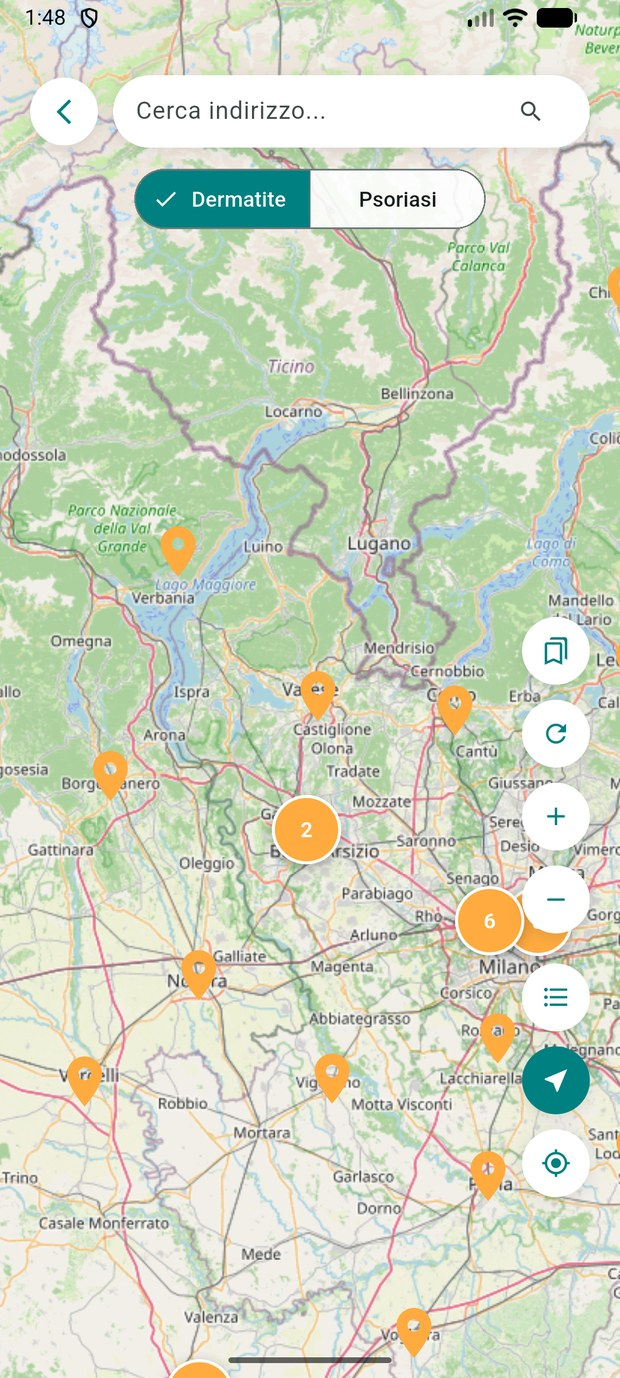
\includegraphics[width=\textwidth]{mappa-cluster}
  \caption*{\scriptsize Cluster in area urbana}
\end{subfigure}
\hfill
\begin{subfigure}[b]{0.27\textwidth}
  \centering
  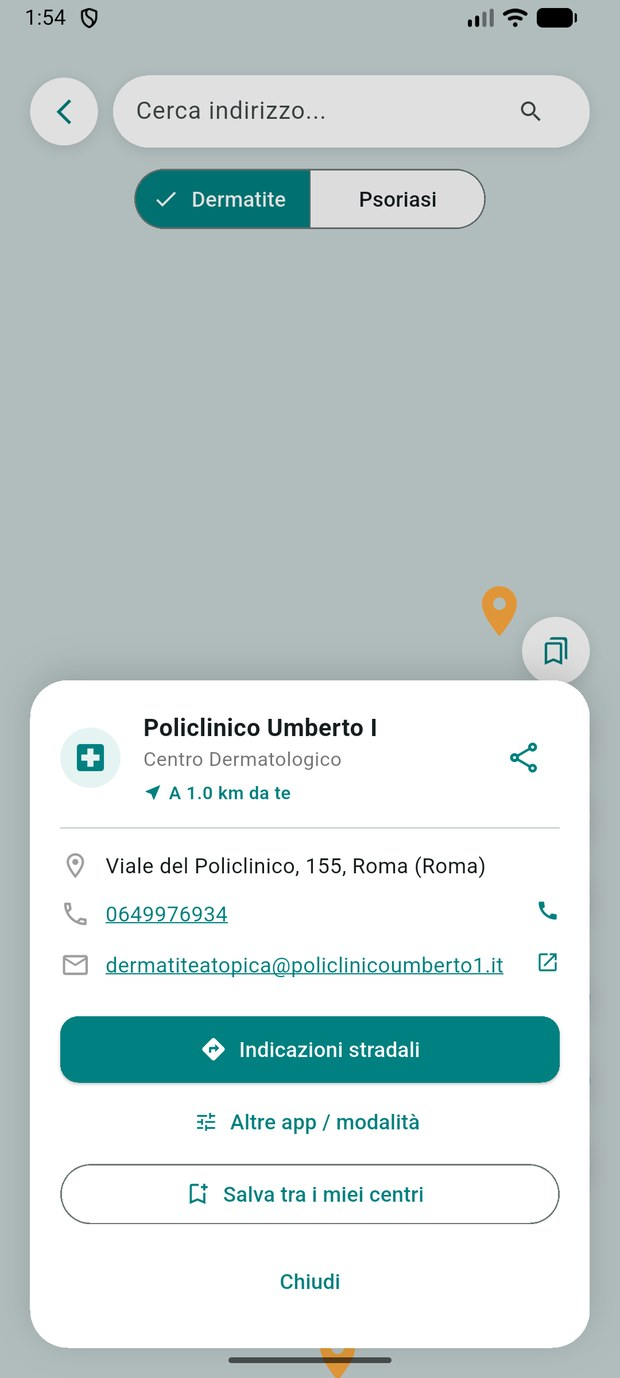
\includegraphics[width=\textwidth]{popup-centro}
  \caption*{\scriptsize Scheda del centro}
\end{subfigure}
\hfill
\begin{subfigure}[b]{0.27\textwidth}
  \centering
  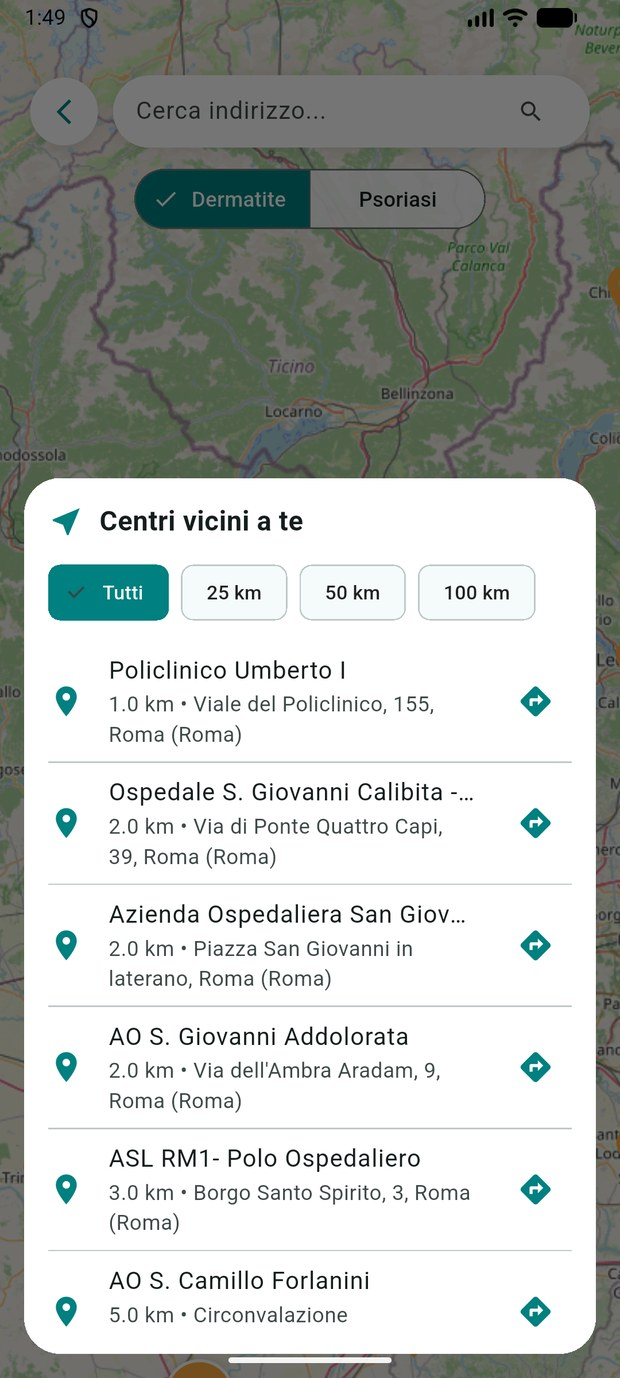
\includegraphics[width=\textwidth]{centri-vicini}
  \caption*{\scriptsize Elenco per distanza}
\end{subfigure}
\caption{L'applicazione: clustering, scheda e ordinamento per distanza.}
\label{fig:sintesi-schermate}
\end{figure}

\section{Verifica e sviluppi futuri}\label{sec:sintesi-verifica}

Quasi tutto dipende da ci\`o che il modulo non controlla: dati di terzi,
posizione ottenuta dal sistema operativo, azioni di altre applicazioni, tile
dalla rete.
Gli Unit Test verificano in modo ripetibile ci\`o che \`e
verificabile, e riserva ai test manuali su emulatore e dispositivo
Android il resto: permessi, cluster, deleghe e assenza di rete.

\begin{table}[H]
\centering
\footnotesize
\begin{tabularx}{\textwidth}{@{}P{4.6cm} P{1.2cm} P{1.6cm}@{}}
\toprule
\textbf{Gruppo di unit test} & \textbf{N.} & \textbf{Esito} \tabularnewline
\midrule
Serializzazione centri personali (campi, null, patologie, coordinate, copia) & 1--5 & Superati \tabularnewline
Archiviazione locale (vuoto, scrittura-lettura, corrotto, forma diversa) & 6--9 & Superati \tabularnewline
Distanze geodetiche (Milano-Roma, null, simmetria) & 10--12 & Superati \tabularnewline
\bottomrule
\end{tabularx}
\caption{Dodici unit test sulla logica applicativa (sintesi).}
\label{tab:sintesi-test}
\end{table}

I dodici unit test coprono serializzazione, persistenza e calcolo
geodetico. %, tutti superati: le letture corrotte restituiscono un elenco
%vuoto, e il caso Milano-Roma assume il valore noto dall'esterno (circa
%477 km con tolleranza di 6 km), rilevando anche un erroneo calcolo euclideo.
Le verifiche manuali coprono permessi, avvio senza rete con e senza cache,
cluster e deleghe. %: tutti superati.

Viene quindi mostrata una mappa funzionante: centri dagli elenchi pubblici con
clustering, filtri per patologia e distanza, voci manuali e delega di
percorso e contatti.
Il problema iniziale viene quindi soddisfatto in due tocchi, e il
contributo non sta solamente nei dati, censiti da altri, ma nell'interrogarli per
prossimit\`a in modo centralizzato.
Restano due limiti: la cache non ha scadenza e il modulo dipende da
elenchi di terzi senza controllo su formato e disponibilit\`a.
Possibili sviluppi futuri: un servizio intermedio che
normalizzi le fonti renderebbe superflue le catene di alias,
rileverebbe i cambiamenti del formato e ridurrebbe le richieste; un meccanismo di sincronizzazione, il quale
richiederebbe cifratura \textit{end-to-end}, perch\'e
l'elenco salvato potrebbe contenere informazioni personali sul paziente; una funzionalità di \textit{routing}
che ordinerebbe i centri per distanza del percorso invece che per distanza in linea d'aria.

% ----------------------
% ---- BIBLIOGRAPHY ----
% ----------------------
% Tutte le voci sono @online: si stampa la sola Sitografia, come nel
% progetto madre, in singola interlinea per restare nelle 10 pagine.
\backmatter
{\singlespacing\sloppy % serve a non far andare i link oltre ai margini
\printbibliography[type=online, heading=bibintoc, title=Sitografia]}

% ----------------------
% ---- DOCUMENT END ----
% ----------------------
\end{document}
